\chapter{Procesamiento de Datos en Tiempo Real}

En los �ltimos tiempos, la demanda de procesamiento de flujos continuos de datos
(data streams) se ha incrementado considerablemente. Esto se debe a que ya no es
suficiente con procesar grandes vol�menes de datos. Los datos, adem�s, deben ser
procesados r�pidamente permitiendo a los sistemas reaccionar ante los eventos lo
antes posible. Ejemplos de sistemas que necesitan �ste nivel de procesamiento
son los sistemas de detecci�n de fraude, monitoreo de recursos, comercio,
etc�tera.

\section{Big Data}

	El t�rmino Big Data, muy utilizado en la actualidad, hace referencia a lo que
	se conoce como las tres V, Volumen, Variedad y Velocidad. Con ello, se quiere
	indicar que un sistema Big Data no solo implica trabajar con grandes vol�menes
	de datos, sino que estos datos pueden ser muy variados y se deben
	procesarr�pidamente.

	\begin{figure}[H]
		\centering
		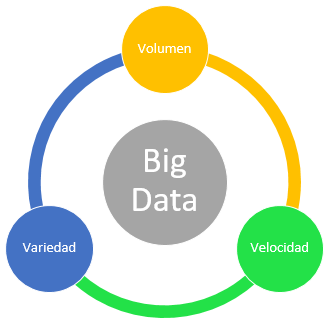
\includegraphics[width=.10\linewidth]{./marco_teorico/img/big_data_tres_v}
	\end{figure}
